\subsection{Progettazione e Codifica}
\subsubsection{I Periodo}
\subsubsubsection{Prospetto orario}
La seguente tabella rappresenta la distribuzione oraria per ogni componente del gruppo nel I periodo della fase di progettazione e codifica:
\begin{table}[H]
\begin{center}
\rowcolors{2}{gray!25}{white}
\renewcommand{\arraystretch}{1.25}
\begin{tabular}{ m{0.20\textwidth}<{\centering}  m{0.06\textwidth}<{\centering} m{0.06\textwidth}<{\centering} m{0.06\textwidth}<{\centering}  m{0.06\textwidth}<{\centering}  m{0.06\textwidth}<{\centering}  m{0.06\textwidth}<{\centering}  m{0.20\textwidth}<{\centering}   }
	\rowcolor{darkblue}
	\textcolor{white}{\textbf{Componente}} &\textcolor{white}{\textbf{Re}}&\textcolor{white}{\textbf{Pt}}&\textcolor{white}{\textbf{An}}&\textcolor{white}{\textbf{Am}}&\textcolor{white}{\textbf{Pr}}&\textcolor{white}{\textbf{Ve}}&\textcolor{white}{\textbf{Ore complessive}}\\ 
	Edoardo Pavan & 0 & 0 & 0 & 2 & 0 & 3 & 5 \\	
	
	Francesco Protopapa & 0 & 0 & 0 & 0 & 0 & 0 & 0 \\

	Greta Cavedon & 1 & 0 & 0 & 0 & 0 & 3 & 4 \\
	
	Luciano Wu & 1 & 0 & 0 & 1 & 0 & 0 & 2 \\
	
	Matteo Basso & 0 & 0 & 2 & 0 & 0 & 2 & 4 \\
	
	Michele Gatto & 1 & 0 & 0 & 0 & 0 & 2 & 3 \\
	
	Pietro Villatora & 0 & 0 & 0 & 0 & 0 & 2 & 2 \\
	
	\textbf{Ore totali ruolo} & 3 & 0 & 2 & 3 & 0 & 12 & 20 \\

\end{tabular}
\caption{Distribuzione oraria per ogni componente nel I periodo della fase di progettazione e codifica}
\end{center}
\end{table}

La tabella può essere rappresentata anche in forma visiva dal seguente grafico:
\begin{figure}[H]
\centering
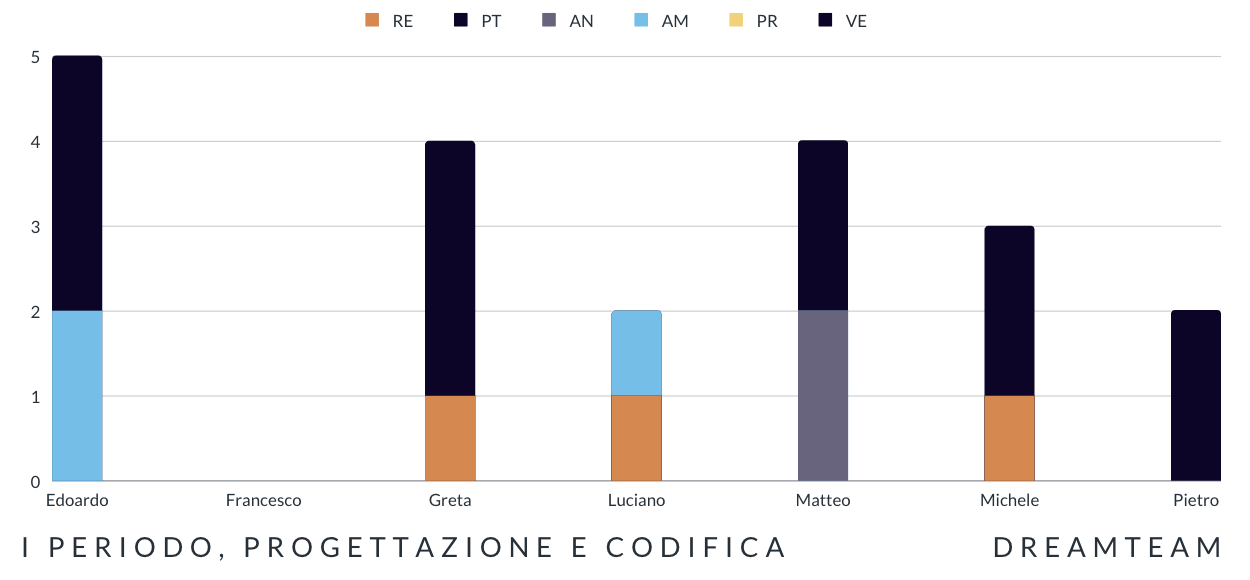
\includegraphics[scale=0.65]{Sezioni/SezioniPreventivo/grafici/Progettazione_codifica_I_periodo.png}
\caption{Istogramma della ripartizione delle ore nel I periodo della fase di progettazione e codifica}
\end{figure}

\subsubsubsection{Prospetto economico}
La seguente tabella rappresenta le ore totali dedicate ad ogni ruolo e il costo in euro:

\begin{table}[H]
\begin{center}
\rowcolors{2}{gray!25}{white}
\renewcommand{\arraystretch}{1.5}
\begin{tabular}{ m{0.3\textwidth}<{\centering}  m{0.2\textwidth}<{\centering} m{0.2\textwidth}<{\centering}}
	\rowcolor{darkblue}
	\textcolor{white}{\textbf{Ruolo}}&\textcolor{white}{\textbf{Totale ore}}&\textcolor{white}{\textbf{Costo totale}}\\ 

	Responsabile  & 3 & 90 \\	
	
	Progettista & 0 & 0 \\
	
	Analista & 2 & 50 \\

	Amministratore & 3 & 60 \\
	
	Programmatore & 0 & 0 \\
	
	Verificatore & 12 & 180 \\
	
	\textbf{Totale} & 20 & 380\euro \\
	
\end{tabular}
\caption{Prospetto del costo per ruoli nel I periodo della fase di progettazione e codifica}
\end{center}
\end{table}

La tabella può essere rappresentata anche in forma visiva dal seguente aerogramma:
\begin{figure}[H]
\centering
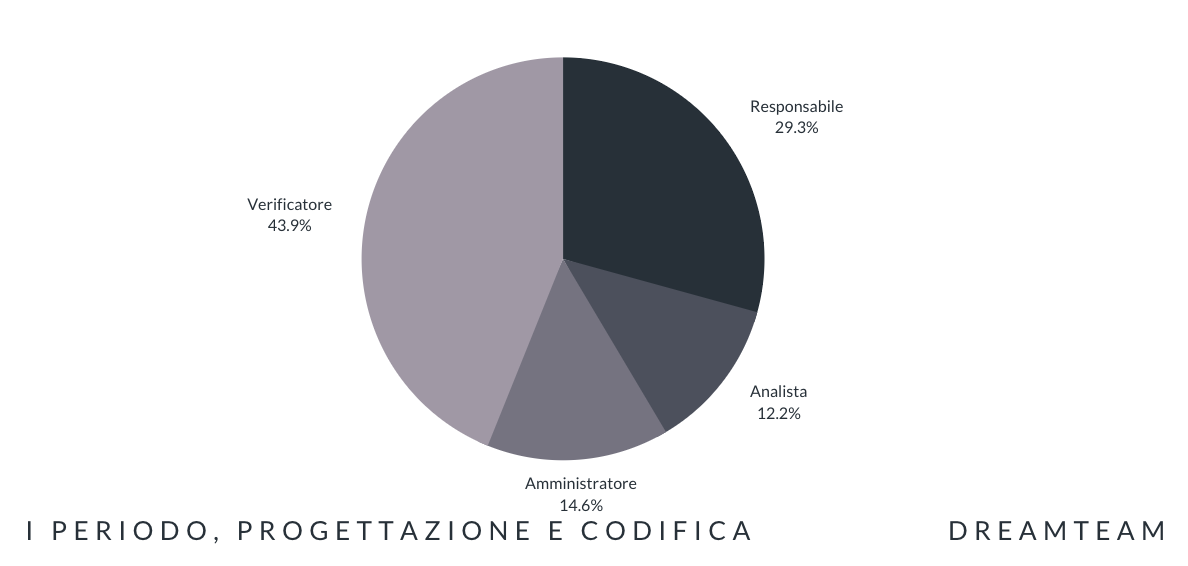
\includegraphics[scale=0.65]{Sezioni/SezioniPreventivo/grafici/Progettazione_I_periodo_costi.png}
\caption{Grafico a torta della ripartizione per ruolo dei costi nel I periodo della fase di progettazione e codifica}
\end{figure}



\subsubsection{II Periodo}
\subsubsubsection{Prospetto orario}
La seguente tabella rappresenta la distribuzione oraria per ogni componente del gruppo nel II periodo della fase di progettazione e codifica:
\begin{table}[H]
\begin{center}
\rowcolors{2}{gray!25}{white}
\renewcommand{\arraystretch}{1.25}
\begin{tabular}{ m{0.20\textwidth}<{\centering}  m{0.06\textwidth}<{\centering} m{0.06\textwidth}<{\centering} m{0.06\textwidth}<{\centering}  m{0.06\textwidth}<{\centering}  m{0.06\textwidth}<{\centering}  m{0.06\textwidth}<{\centering}  m{0.20\textwidth}<{\centering}   }
	\rowcolor{darkblue}
	\textcolor{white}{\textbf{Componente}} &\textcolor{white}{\textbf{Re}}&\textcolor{white}{\textbf{Pt}}&\textcolor{white}{\textbf{An}}&\textcolor{white}{\textbf{Am}}&\textcolor{white}{\textbf{Pr}}&\textcolor{white}{\textbf{Ve}}&\textcolor{white}{\textbf{Ore complessive}}\\ 
	Edoardo Pavan & 1 & 9 & 0 & 2 & 0 & 2 & 14 \\	
	
	Francesco Protopapa & 1 & 6 & 0 & 0 & 0 & 2 & 9 \\

	Greta Cavedon & 1 & 6 & 0 & 0 & 0 & 2 & 9 \\
	
	Luciano Wu & 2 & 3 & 0 & 1 & 0 & 2 & 8 \\
	
	Matteo Basso & 0 & 3 & 3 & 0 & 0 & 2 & 8 \\
	
	Michele Gatto & 2 & 3 & 0 & 0 & 0 & 1 & 6 \\
	
	Pietro Villatora & 0 & 3 & 0 & 1 & 0 & 2 & 6 \\
	
	\textbf{Ore totali ruolo} & 7 & 33 & 3 & 4 & 0 & 13 & 60 \\

\end{tabular}
\caption{Distribuzione oraria per ogni componente nel II periodo della fase di progettazione e codifica}
\end{center}
\end{table}

La tabella può essere rappresentata anche in forma visiva dal seguente grafico:
\begin{figure}[H]
\centering
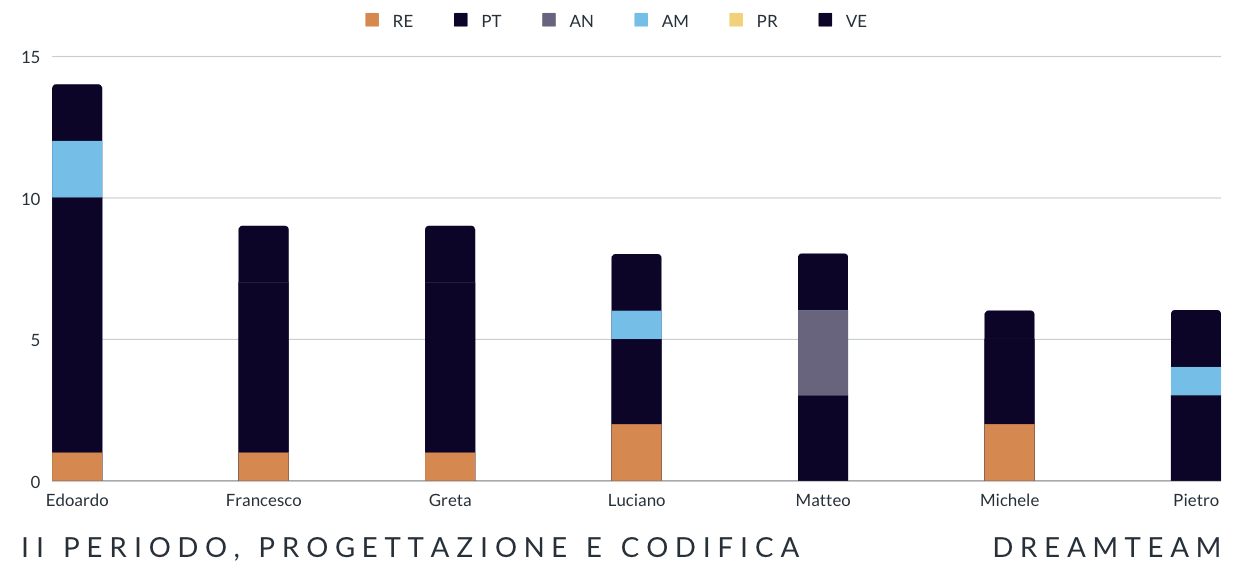
\includegraphics[scale=0.65]{Sezioni/SezioniPreventivo/grafici/Progettazione_codifica_II_periodo.png}
\caption{Istogramma della ripartizione delle ore nel II periodo della fase di progettazione e codifica}
\end{figure}

\subsubsubsection{Prospetto economico}
La seguente tabella rappresenta le ore totali dedicate ad ogni ruolo e il costo in euro:

\begin{table}[H]
\begin{center}
\rowcolors{2}{gray!25}{white}
\renewcommand{\arraystretch}{1.5}
\begin{tabular}{ m{0.3\textwidth}<{\centering}  m{0.2\textwidth}<{\centering} m{0.2\textwidth}<{\centering}}
	\rowcolor{darkblue}
	\textcolor{white}{\textbf{Ruolo}}&\textcolor{white}{\textbf{Totale ore}}&\textcolor{white}{\textbf{Costo totale}}\\ 

	Responsabile  & 7 & 210 \\	
	
	Progettista & 33 & 825 \\
	
	Analista & 3 & 75 \\

	Amministratore & 4 & 80 \\
	
	Programmatore & 0 & 0 \\
	
	Verificatore & 13 & 195 \\
	
	\textbf{Totale} & 60 & 1385\euro \\
	
\end{tabular}
\caption{Prospetto del costo per ruoli nel II periodo della fase di progettazione e codifica}
\end{center}
\end{table}

La tabella può essere rappresentata anche in forma visiva dal seguente aerogramma:

\begin{figure}[H]
\centering
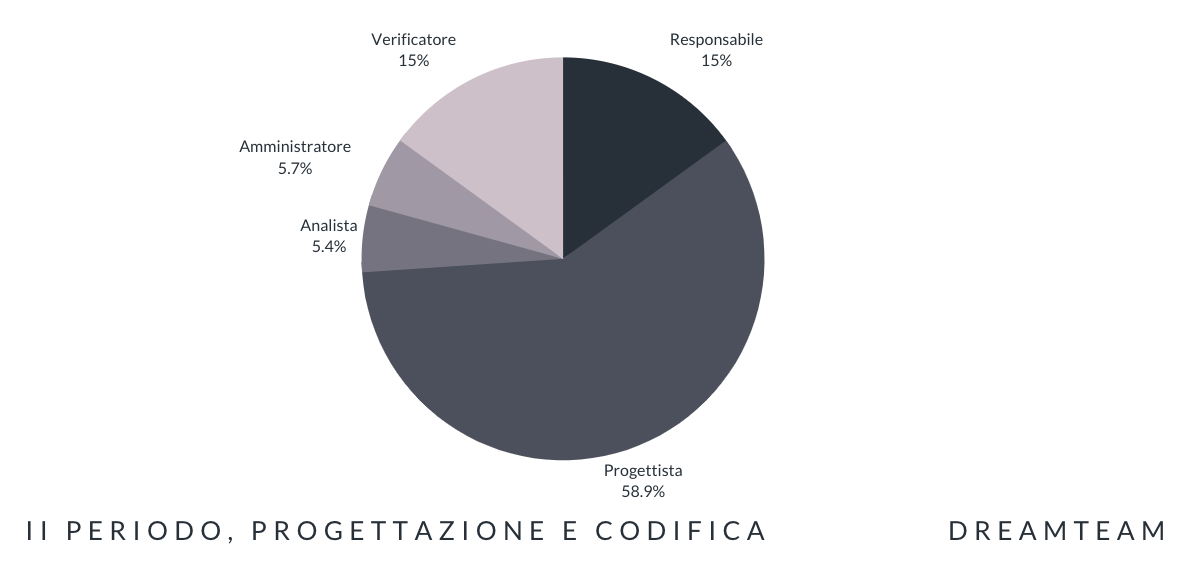
\includegraphics[scale=0.65]{Sezioni/SezioniPreventivo/grafici/Progettazione_II_periodo_costi.png}
\caption{Grafico a torta della ripartizione per ruolo dei costi nel II periodo della fase di progettazione e codifica}
\end{figure}


\subsubsection{III Periodo}
\subsubsubsection{Prospetto orario}
La seguente tabella rappresenta la distribuzione oraria per ogni componente del gruppo nel III periodo della fase di progettazione e codifica:
\begin{table}[H]
\begin{center}
\rowcolors{2}{gray!25}{white}
\renewcommand{\arraystretch}{1.25}
\begin{tabular}{ m{0.20\textwidth}<{\centering}  m{0.06\textwidth}<{\centering} m{0.06\textwidth}<{\centering} m{0.06\textwidth}<{\centering}  m{0.06\textwidth}<{\centering}  m{0.06\textwidth}<{\centering}  m{0.06\textwidth}<{\centering}  m{0.20\textwidth}<{\centering}   }
	\rowcolor{darkblue}
	\textcolor{white}{\textbf{Componente}} &\textcolor{white}{\textbf{Re}}&\textcolor{white}{\textbf{Pt}}&\textcolor{white}{\textbf{An}}&\textcolor{white}{\textbf{Am}}&\textcolor{white}{\textbf{Pr}}&\textcolor{white}{\textbf{Ve}}&\textcolor{white}{\textbf{Ore complessive}}\\ 
	Edoardo Pavan & 1 & 2 & 0 & 2 & 11 & 4 & 20 \\	
	
	Francesco Protopapa & 1 & 1 & 0 & 0 & 10 & 2 & 14 \\

	Greta Cavedon & 0 & 0 & 0 & 0 & 8 & 4 & 12 \\
	
	Luciano Wu & 2 & 3 & 0 & 1 & 8 & 2 & 16 \\
	
	Matteo Basso & 0 & 3 & 2 & 0 & 7 & 1 & 13 \\
	
	Michele Gatto & 1  & 2 & 0 & 0 & 10 & 0 & 13 \\
	
	Pietro Villatora & 0 & 2 & 0 & 1 & 16 & 0 & 19 \\
	
	\textbf{Ore totali ruolo} & 5 & 13 & 2 & 4 & 70 & 13 & 107 \\

\end{tabular}
\caption{Distribuzione oraria per ogni componente nel III periodo della fase di progettazione e codifica}
\end{center}
\end{table}

La tabella può essere rappresentata anche in forma visiva dal seguente grafico:
\begin{figure}[H]
\centering
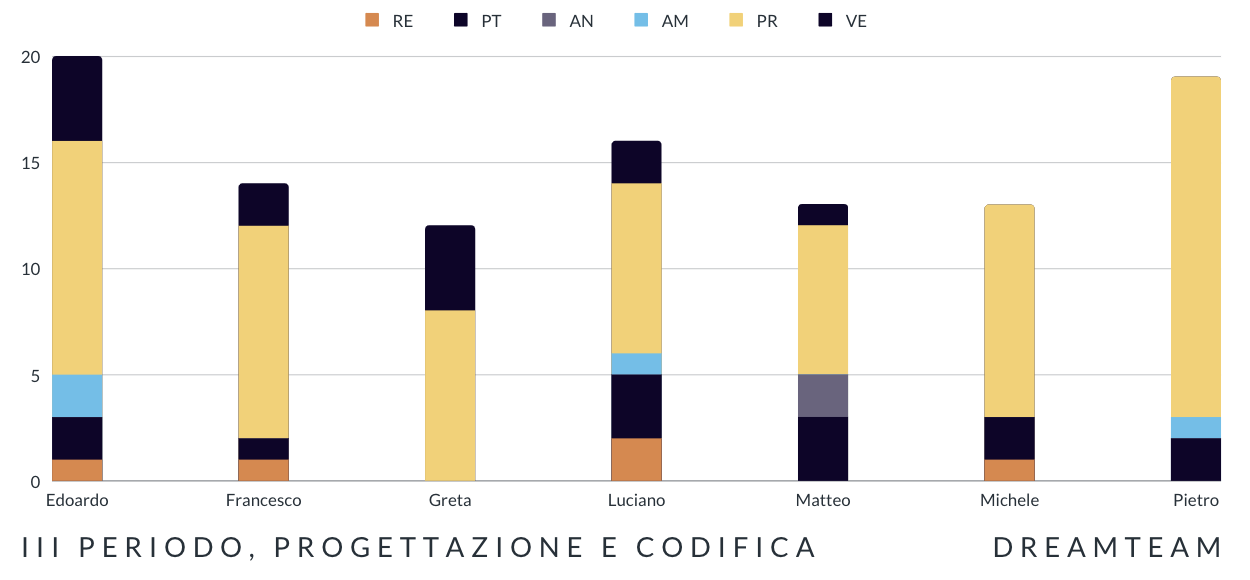
\includegraphics[scale=0.65]{Sezioni/SezioniPreventivo/grafici/Progettazione_codifica_III_periodo.png}
\caption{Istogramma della ripartizione delle ore nel III periodo della fase di progettazione e codifica}
\end{figure}

\subsubsubsection{Prospetto economico}
La seguente tabella rappresenta le ore totali dedicate ad ogni ruolo e il costo in euro:

\begin{table}[H]
\begin{center}
\rowcolors{2}{gray!25}{white}
\renewcommand{\arraystretch}{1.5}
\begin{tabular}{ m{0.3\textwidth}<{\centering}  m{0.2\textwidth}<{\centering} m{0.2\textwidth}<{\centering}}
	\rowcolor{darkblue}
	\textcolor{white}{\textbf{Ruolo}}&\textcolor{white}{\textbf{Totale ore}}&\textcolor{white}{\textbf{Costo totale}}\\ 

	Responsabile  & 5 & 150 \\	
	
	Progettista & 13 & 325 \\
	
	Analista & 2 & 50 \\

	Amministratore & 4 & 80 \\
	
	Programmatore & 70 & 1050 \\
	
	Verificatore & 13 & 195 \\
	
	\textbf{Totale} & 107 & 1850\euro \\
	
\end{tabular}
\caption{Prospetto del costo per ruoli nel III periodo della fase di progettazione e codifica}
\end{center}
\end{table}

La tabella può essere rappresentata anche in forma visiva dal seguente aerogramma:
\begin{figure}[H]
\centering
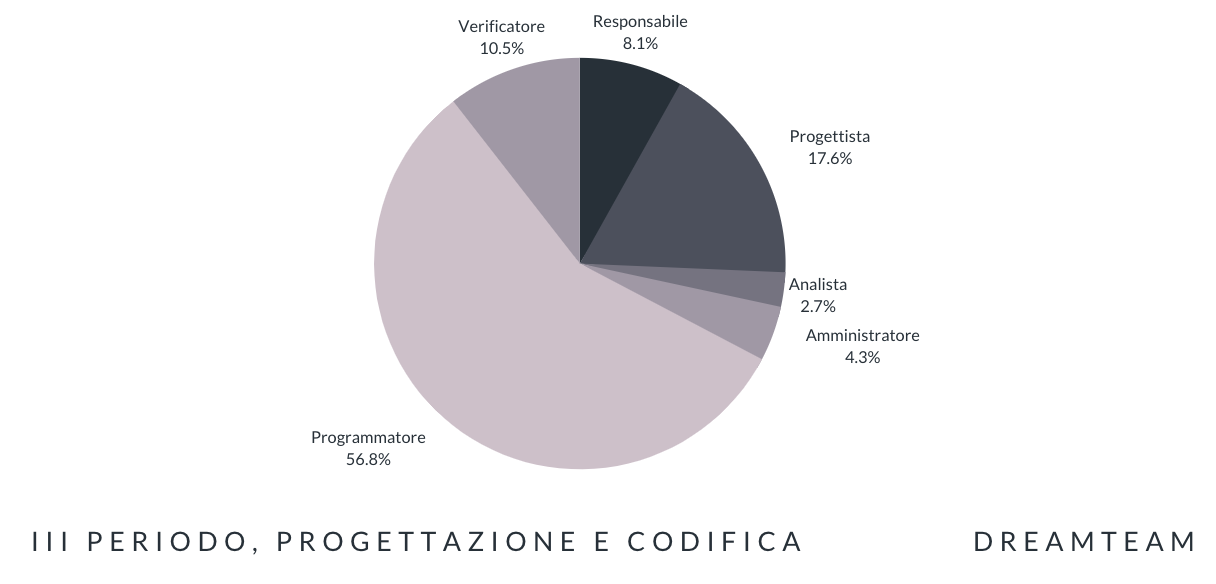
\includegraphics[scale=0.65]{Sezioni/SezioniPreventivo/grafici/Progettazione_III_periodo_costi.png}
\caption{Grafico a torta della ripartizione per ruolo dei costi nel III periodo della fase di progettazione e codifica}
\end{figure}



\subsubsection{IV Periodo}
\subsubsubsection{Prospetto orario}
La seguente tabella rappresenta la distribuzione oraria per ogni componente del gruppo nel IV periodo della fase di progettazione e codifica:
\begin{table}[H]
\begin{center}
\rowcolors{2}{gray!25}{white}
\renewcommand{\arraystretch}{1.25}
\begin{tabular}{ m{0.20\textwidth}<{\centering}  m{0.06\textwidth}<{\centering} m{0.06\textwidth}<{\centering} m{0.06\textwidth}<{\centering}  m{0.06\textwidth}<{\centering}  m{0.06\textwidth}<{\centering}  m{0.06\textwidth}<{\centering}  m{0.20\textwidth}<{\centering}   }
	\rowcolor{darkblue}
	\textcolor{white}{\textbf{Componente}} &\textcolor{white}{\textbf{Re}}&\textcolor{white}{\textbf{Pt}}&\textcolor{white}{\textbf{An}}&\textcolor{white}{\textbf{Am}}&\textcolor{white}{\textbf{Pr}}&\textcolor{white}{\textbf{Ve}}&\textcolor{white}{\textbf{Ore complessive}}\\ 
	Edoardo Pavan & 0 & 2 & 0 & 1 & 11 & 1 & 15 \\	
	
	Francesco Protopapa & 0 & 1 & 0 & 1 & 10 & 2 & 14 \\

	Greta Cavedon & 1 & 1 & 0 & 0 & 8 & 1 & 11 \\
	
	Luciano Wu & 0 & 4 & 0 & 1 & 8 & 2 & 15 \\
	
	Matteo Basso & 0 & 3 & 3 & 0 & 8 & 2 & 16 \\
	
	Michele Gatto & 2  & 3 & 0 & 0 & 10 & 2 & 17 \\
	
	Pietro Villatora & 0 & 3 & 0 & 0 & 15 & 2 & 20 \\
	
	\textbf{Ore totali ruolo} & 3 & 17 & 3 & 3 & 70 & 12 & 108 \\

\end{tabular}
\caption{Distribuzione oraria per ogni componente nel IV periodo della fase di progettazione e codifica}
\end{center}
\end{table}

La tabella può essere rappresentata anche in forma visiva dal seguente grafico:
\begin{figure}[H]
\centering
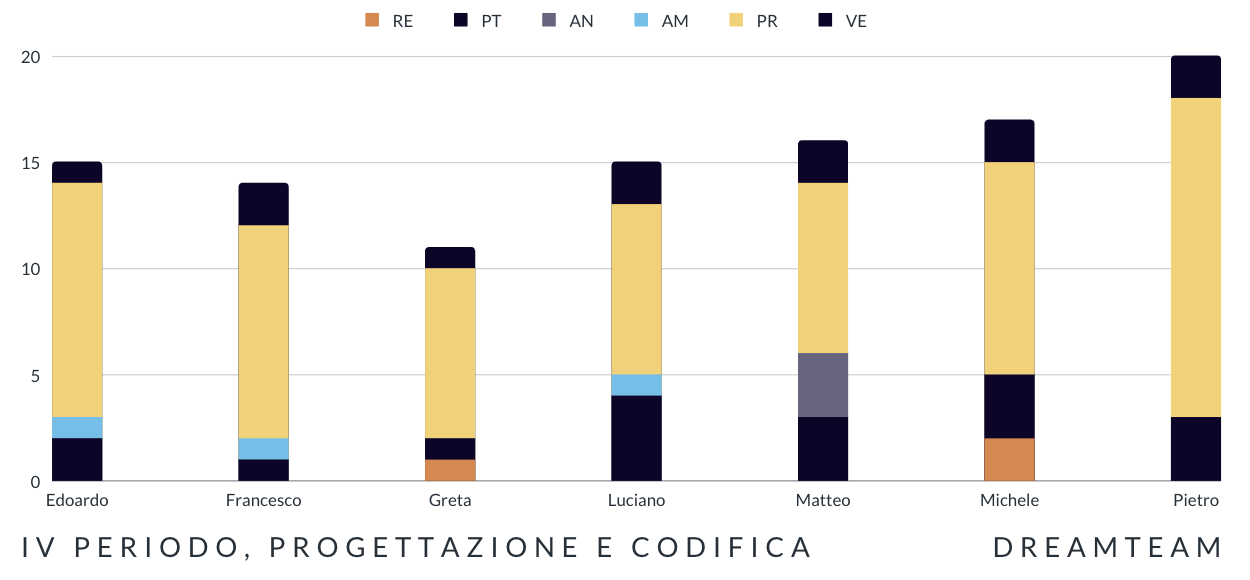
\includegraphics[scale=0.65]{Sezioni/SezioniPreventivo/grafici/Progettazione_codifica_IV_periodo.png}
\caption{Istogramma della ripartizione delle ore nel IV periodo della fase di progettazione e codifica}
\end{figure}

\subsubsubsection{Prospetto economico}
La seguente tabella rappresenta le ore totali dedicate ad ogni ruolo e il costo in euro:

\begin{table}[H]
\begin{center}
\rowcolors{2}{gray!25}{white}
\renewcommand{\arraystretch}{1.5}
\begin{tabular}{ m{0.3\textwidth}<{\centering}  m{0.2\textwidth}<{\centering} m{0.2\textwidth}<{\centering}}
	\rowcolor{darkblue}
	\textcolor{white}{\textbf{Ruolo}}&\textcolor{white}{\textbf{Totale ore}}&\textcolor{white}{\textbf{Costo totale}}\\ 

	Responsabile  & 3 & 90 \\	
	
	Progettista & 17 & 425 \\
	
	Analista & 3 & 75 \\

	Amministratore & 3 & 60 \\
	
	Programmatore & 70 & 1050 \\
	
	Verificatore & 12 & 180 \\
	
	\textbf{Totale} & 108 & 1880\euro \\
	
\end{tabular}
\caption{Prospetto del costo per ruoli nel IV periodo della fase di progettazione e codifica}
\end{center}
\end{table}

La tabella può essere rappresentata anche in forma visiva dal seguente aerogramma:
\begin{figure}[H]
\centering
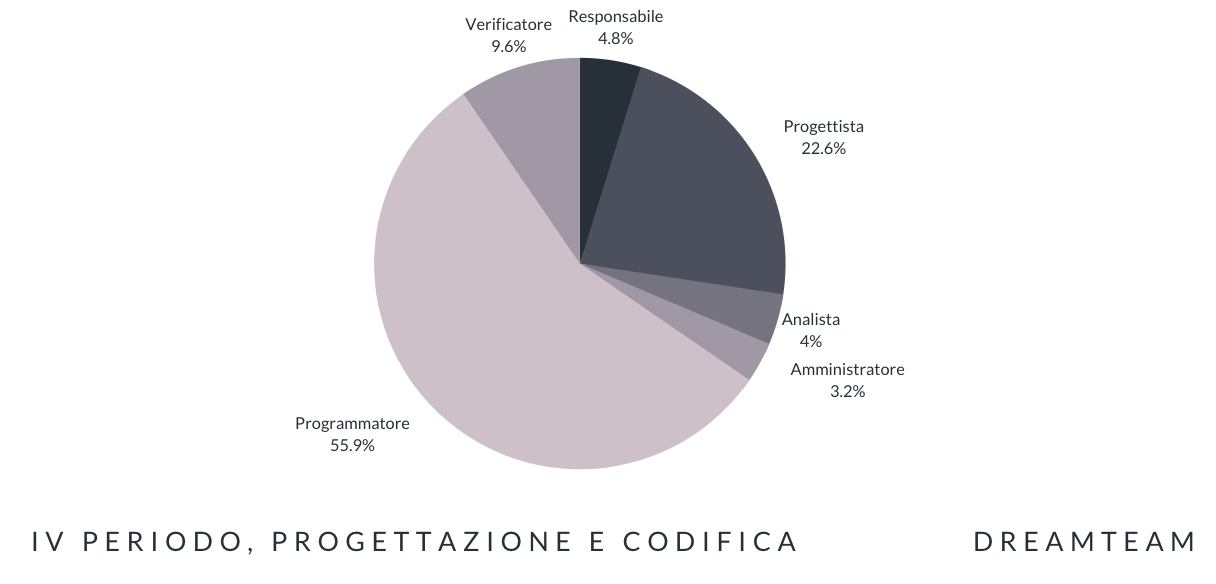
\includegraphics[scale=0.65]{Sezioni/SezioniPreventivo/grafici/Progettazione_IV_periodo_costi.png}
\caption{Grafico a torta della ripartizione per ruolo dei costi nel IV periodo della fase di progettazione e codifica}
\end{figure}


\subsubsection{Fase complessiva}
\subsubsubsection{Prospetto orario}
La seguente tabella rappresenta la distribuzione oraria per ogni componente del gruppo nella fase di progettazione e codifica:
\begin{table}[H]
\begin{center}
\rowcolors{2}{gray!25}{white}
\renewcommand{\arraystretch}{1.25}
\begin{tabular}{ m{0.20\textwidth}<{\centering}  m{0.06\textwidth}<{\centering} m{0.06\textwidth}<{\centering} m{0.06\textwidth}<{\centering}  m{0.06\textwidth}<{\centering}  m{0.06\textwidth}<{\centering}  m{0.06\textwidth}<{\centering}  m{0.20\textwidth}<{\centering}   }
	\rowcolor{darkblue}
	\textcolor{white}{\textbf{Componente}} &\textcolor{white}{\textbf{Re}}&\textcolor{white}{\textbf{Pt}}&\textcolor{white}{\textbf{An}}&\textcolor{white}{\textbf{Am}}&\textcolor{white}{\textbf{Pr}}&\textcolor{white}{\textbf{Ve}}&\textcolor{white}{\textbf{Ore complessive}}\\ 
	Edoardo Pavan & 2 & 13 & 0 & 7 & 22 & 10 & 54 \\	
	
	Francesco Protopapa & 2 & 8 & 0 & 1 & 20 & 6 & 37 \\

	Greta Cavedon & 3 & 7 & 0 & 0 & 16 & 10 & 36 \\
	
	Luciano Wu & 5 & 10 & 0 & 4 & 16 & 6 & 41 \\
	
	Matteo Basso & 0 & 9 & 10 & 0 & 15 & 7 & 41 \\
	
	Michele Gatto &  6 & 8 & 0 & 0 & 20 & 5 & 39 \\
	
	Pietro Villatora & 0 & 8 & 0 & 2 & 31 & 6 & 47 \\
	
	\textbf{Ore totali ruolo} & 18 & 63 & 10 & 14 & 140 & 50 & 295\\

\end{tabular}
\caption{Distribuzione oraria per ogni componente nella fase di progettazione e codifica}
\end{center}
\end{table}

La tabella può essere rappresentata anche in forma visiva dal seguente grafico:
\begin{figure}[H]
\centering
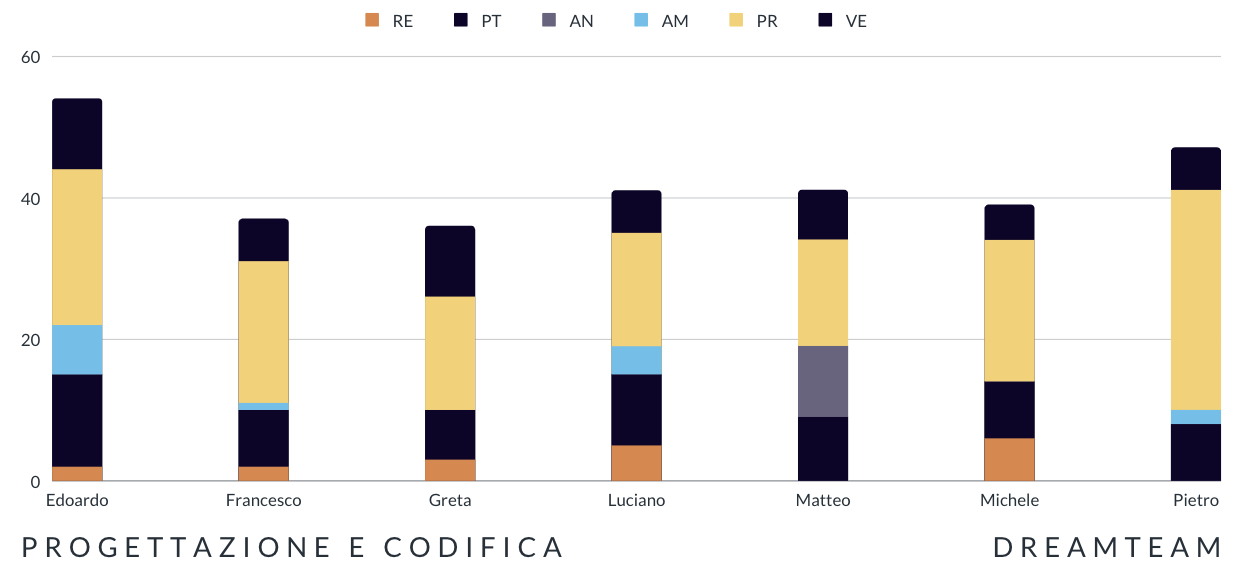
\includegraphics[scale=0.65]{Sezioni/SezioniPreventivo/grafici/Progettazione_codifica.png}
\caption{Istogramma della ripartizione delle ore nella fase di progettazione e codifica}
\end{figure}

\subsubsubsection{Prospetto economico}
La seguente tabella rappresenta le ore totali dedicate ad ogni ruolo e il costo in euro:

\begin{table}[H]
\begin{center}
\rowcolors{2}{gray!25}{white}
\renewcommand{\arraystretch}{1.5}
\begin{tabular}{ m{0.3\textwidth}<{\centering}  m{0.2\textwidth}<{\centering} m{0.2\textwidth}<{\centering}}
	\rowcolor{darkblue}
	\textcolor{white}{\textbf{Ruolo}}&\textcolor{white}{\textbf{Totale ore}}&\textcolor{white}{\textbf{Costo totale}}\\ 

	Responsabile  & 18 & 540 \\	
	
	Progettista & 63 & 1575 \\
	
	Analista & 10 & 250 \\

	Amministratore & 14 & 280 \\
	
	Programmatore & 140 & 2100 \\
	
	Verificatore & 50 & 750 \\
	
	\textbf{Totale} & 295 & 5495\euro \\
	
\end{tabular}
\caption{Prospetto del costo per ruoli nella fase di progettazione e codifica}
\end{center}
\end{table}

La tabella può essere rappresentata anche in forma visiva dal seguente aerogramma:
\begin{figure}[H]
\centering
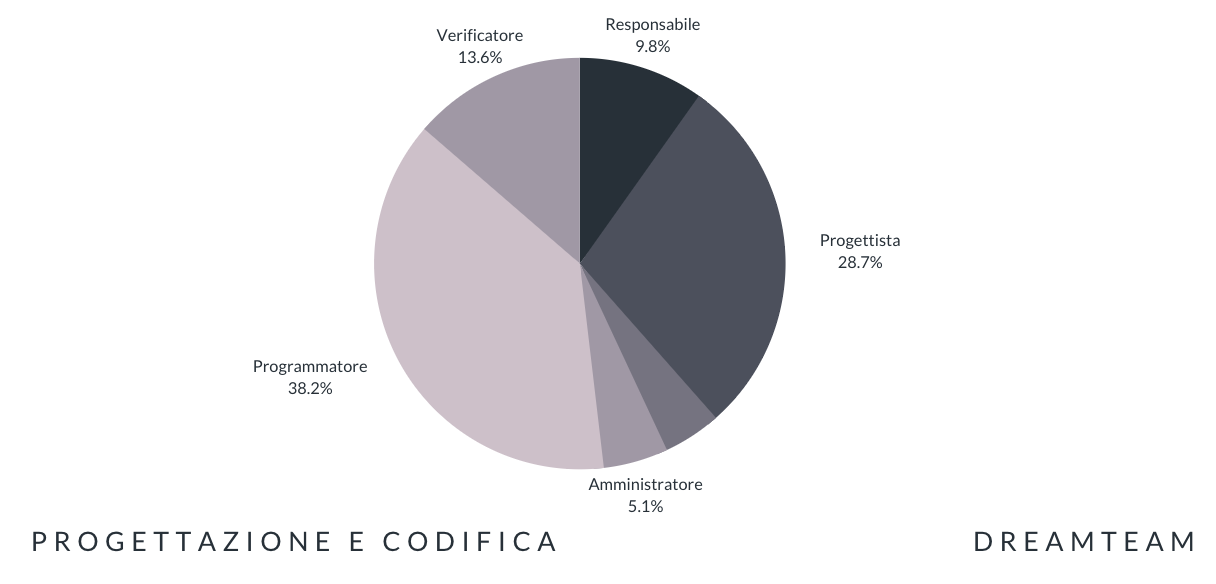
\includegraphics[scale=0.65]{Sezioni/SezioniPreventivo/grafici/Progettazione_costi.png}
\caption{Grafico a torta della ripartizione per ruolo dei costi nella fase di progettazione e codifica}
\end{figure}



